% !TEX root = ../../../main.tex

\toggletrue{image}
\toggletrue{imagehover}
\chapterimage{cryptography}
\chapterimagetitle{\uppercase{Cryptography}}
\chapterimageurl{https://xkcd.com/153/}
\chapterimagehover{If you got a big keyspace, let me search it.}

\chapter{Grundlagen}
\label{chapter-sym-kryptosysteme-grundlagen}

Wir verbessern das Prinzip von Geheimschriften, in dem wir mehrere \say{Geheimnisse} zur Verfügung stellen. Sender und Empfänger einigen sich dann auf eines der Geheimnisse. Diese Idee verfolgen symmetrische Kryptosysteme. Die Lernziele lauten:

\newcommand{\grundlagenSymmetrischeKryptosystemeLernziele}{
\protect\begin{todolist}
\item Sie erklären das Kommunikationsszenario für symmetrische Kryptosysteme.
\item Sie erklären, was wir unter einem Schlüssel verstehen.
\item Sie definieren das Sicherheitskriterium für symmetrische Kryptosysteme.
\end{todolist}
}

\lernziel{\autoref{chapter-sym-kryptosysteme-grundlagen}, \nameref{chapter-sym-kryptosysteme-grundlagen}}{\protect\grundlagenSymmetrischeKryptosystemeLernziele}

\grundlagenSymmetrischeKryptosystemeLernziele

\section{Kommunikationsszenario}

Wir erweitern das bisherige Kommunikationsszenario für Geheimschriften und führen neue Fachbegriffe ein. \autoref{figure-kommunikationsszenario-symmetrische-kryptosysteme} zeigt die Details der Kommunikation für symmetrische Kryptosysteme.

\begin{figure}[htb]
\centering
\begin{tikzpicture}
\node [cloud, draw, cloud puffs=7, cloud puff arc=120, aspect=3, text width=2.5cm, align=center] (medium) at (0,0) {\footnotesize Übertragungsmedium};

\node[inner sep=0pt] (alice) at (-6,2)
    {
\includegraphics[scale=0.25]{alice_tiny}};
\node[text width=2cm, align=center] (sender) at (-5, 2) {Sender (Alice)};
\node[rectangle, fill=black!25] (ver) at (-5.5, 0) {Verschlüsselung};
\draw[-latex, very thick] (alice.south west) -- (ver.north) node[left, midway] {Klartext};
\draw[-latex, very thick] (sender.south) -- (ver.north) node[right, midway] {Schlüssel};
\draw[-latex, very thick] (ver.east) -- (medium.west) node[above, midway] {Kryptotext};

\node[inner sep=0pt] (bob) at (5,2)
    {
\includegraphics[scale=0.25]{bob_tiny}};
\node[text width=2cm, align=left] (empfaenger) at (6.5, 2) {Empfänger (Bob)};
\node[rectangle, fill=black!25] (entsch) at (5.5, 0) {Entschlüsselung};
\draw[-latex, very thick] (entsch.north) -- (5.5, 1.5) node[right, midway] {Klartext};
\draw[-latex, very thick] (5, 1.5) -- (5, 0.25) node[left, midway] {Schlüssel};
\draw[-latex, very thick] (medium.east) -- (entsch.west) node[above, midway] {Kryptotext};

\node[inner sep=0pt] (eve) at (-0.75,-2.5)
    {
\includegraphics[scale=0.25]{eve_tiny}};
\node[text width=3cm, align=center] (pangreifer) at (0.75, -2.5) {Passiver Angreifer (Eve)};
\draw[-latex, very thick] (medium.south) -- (0, -2) node[right, midway] {Kryptotext (Kopie)};

\end{tikzpicture}
\caption{Kommunikationsszenario bei symmetrischen Kryptosystemen.}
\label{figure-kommunikationsszenario-symmetrische-kryptosysteme}
\end{figure}

Bei Kryptosystemen sprechen wir nun von \textbf{Verschlüsselung} anstelle von Chiffrierung, um deutlich zu machen, dass der Klartext mit einem \textbf{Schlüssel} transformiert wird. Das Ergebnis der Verschlüsselung nennen wir deshalb auch \textbf{Kryptotext}. Ein Kryptotext wird jetzt nicht mehr dechiffriert, sondern es wird mit einem Schlüssel eine \textbf{Entschlüsselung} durchgeführt. Auf die gleiche Weise passen wir die Begriffe für die Alphabete an. Wir verwenden den Begriff \textbf{Kryptotextalphabet}, wenn wir die Zeichen aus denen ein Kryptotext bestehen kann, angeben möchten. Klartextalphabet und Kryptotextalphabet müssen auch bei Kryptosystemen nicht identisch sein.

\section{Geheimschriften versus symmetrische Kryptosysteme}

Alle Kryptosysteme basieren auf der Idee, dass das \textbf{Verfahren zur Verschlüsselung und Entschlüsselung öffentlich bekannt} ist. Ein Kryptograph\footnote{Ein Entwickler eines Kryptosystems.} darf somit nicht annehmen, dass das Kryptosystem geheim bleibt und Eve das Verfahren nicht kennt. Bei Geheimschriften dürfen nur Alice und Bob die Verfahren zur Chiffrierung und Dechiffrierung kennen. Da wir bei Kryptosystemen dies nun preisgeben, benötigen Alice und Bob einen \textbf{anderen Wissensvorsprung} gegenüber Eve. Dies ist bei symmetrischen Kryptosystemen der \textbf{Schlüssel}.

\begin{hinweis}
	Ein Kryptosystem mit einem fixen Schlüssel entspricht einer Geheimschrift. Die Terminologie (Geheimschrift und Kryptosystem) wird in der Literatur unterschiedlich gehandhabt.
\end{hinweis}

\section{Schlüssel}

Der Schlüssel stellt die \textbf{exklusive Information} zwischen Alice und Bob dar.

\begin{definition}[Symmetrische Kryptosysteme]
	Verfügen in einem Kryptosystem Alice und Bob über den \textbf{gleichen} Schlüssel und dieser Schlüssel wird sowohl zum \textbf{Verschlüsseln}, als auch zum \textbf{Entschlüsseln} benutzt, dann handelt es sich um ein symmetrisches Kryptosystem.
\end{definition}

Alice und Bob müssen sich \textbf{vor} der Kommunikation auf einen gemeinsamen Schlüssel einigen. Nur dann kann Bob mit dem Schlüssel aus dem Kryptotext wieder den Klartext erzeugen.

\begin{example}
Beispiele für einen Schlüssel: eine \textbf{Folge von Zeichen} (Buchstaben, Zahlen etc.), eine \textbf{Tabelle} oder eine \textbf{Folge von Bits}.
\end{example}

In \autoref{figure-kommunikationsszenario-symmetrische-kryptosysteme} besitzen somit Alice und Bob den gleichen Schlüssel. Eve erhält weiterhin eine Kopie des Kryptotexts und hat die Aufgabe, den Klartext herauszufinden.

\begin{important}
	Allein durch den \textbf{Kryptotext} und die \textbf{Beschreibung des Kryptosystems} versucht Eve den Klartext zu ermitteln. Falls dies gelingt, dann wurde das Kryptosystem \say{geknackt} und gilt als nicht sicher.
\end{important}

\begin{definition}[Schlüsselmenge]
Die Schlüsselmenge $\mathscr{S}$ beschreibt alle möglichen Schlüssel, welche für ein Kryptosystem gewählt werden können. Die Anzahl der verschiedenen Schlüssel bezeichnen wir mit $|\mathscr{S}|$.
\end{definition}

\subsection{Warum den Schlüssel festlegen?}

Die Schlüsselfestlegung muss auf einem \say{sicheren Weg} passieren, sodass Eve nicht an den Schlüssel kommt. Dabei können wir uns fragen, warum überhaupt erst den Schlüssel auf einem \say{sicheren Weg} abmachen und nicht gleich den Klartext darüber übermitteln. Zwei Anmerkungen dazu:

\begin{itemize}
	\item Alice und Bob können den Schlüssel unabhängig von der Nachrichtenübertragung abmachen. Dies kann auch zeitlich voneinander losgekoppelt sein. Der Schlüssel kann zum Beginn des Monats werden und die Nachricht kann \say{spontan} übertragen werden.
	\item Oft hat ein Schlüssel eine feste Länge (z.B. für den Schlüssel wird immer ein Wort mit 20 Buchstaben verwendet oder eine Folge von 128 Bits). Dadurch reduziert sich der Aufwand für die Schlüsselfestlegung im Vergleich zu einem Klartext mit variabler Länge. 
\end{itemize}

Es bleibt nun offen, wie Alice und Bob über einen \say{sicheren Weg} den Schlüssel festlegen. Wir kümmern uns um diese Antwort in einem separaten Kapitel (Schlüsselfestlegung). Bis dahin, gehen wir stets davon aus, dass Alice und Bob über den gleichen Schlüssel verfügen.

\section{Sicherheit}

Konstruieren wir ein neues Kryptosystem, dann ist die Sicherheit von zentraler Bedeutung. 

\begin{important}
Unter einem sicheren Kryptosystem stellen wir uns \textbf{intuitiv} ein System vor, bei dem ein Kryptotext \textbf{ohne} die Kenntnis des \textbf{Schlüssels} nicht geknackt werden kann.
\end{important}

Diese Intuition hat der niederländische  Linguist und Kryptologe Auguste Kerkhoff im 19. Jahrhundert wie folgt formalisiert:

\begin{definition}[Kerkhoffs-Prinzip der Sicherheit]
Die Sicherheit eines Kryptosystems darf \textbf{nicht} von der \textbf{Geheimhaltung} der \textbf{Verschlüsselungs- und Entschlüsselungsverfahren} abhängen. Die Sicherheit gründet sich \textbf{nur} auf die \textbf{Geheimhaltung} des \textbf{Schlüssels}. Das Kryptosystem ist sicher, wenn sich der ursprüngliche Klartext nicht ohne die Kenntnis des Schlüssels aus einem oder mehreren Kryptotexten ableiten lässt.
\end{definition}

Wir gehen also ab sofort davon aus, dass das Verschlüsselungs- und Entschlüsselungsverfahren jeder Person bekannt ist -- es ist \textbf{nicht} geheim. Wir können die \textbf{Unsicherheit} eines Kryptosystems zeigen, in dem wir für einen Kryptotext entweder den Klartext herausfinden oder Informationen über den Schlüssel ermitteln. Dieser Vorgang nennt sich \textbf{Attacke} oder \textbf{Angriff} auf das Kryptosystem.

\begin{definition}[Angriff mit bekanntem Kryptotext]
Kennt der Kryptoanalytiker den Kryptotext oder einen relativ grossen Teil davon und möchte damit das Kryptosystem knacken, dann sprechen wir von einem Angriff mit bekanntem Kryptotext (eng. known ciphertext attack). Dies ist eine realistische Annahme, da wir relativ einfach einen Kryptotext erhalten können (z.B. Abhören von Daten im \ac{WLAN}).
\end{definition}

\vfill

\begin{figure}[htb]
\centering
\caption*{\uppercase{Encryption} \\ \url{https://xkcd.com/2691/}}
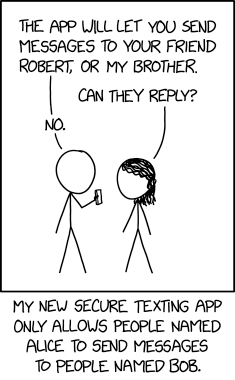
\includegraphics[scale=0.75]{encryption}
\caption*{\uppercase{WARNING: PEOPLE NAMED EVE ARE PROHIBITED FROM INSTALLING THIS APP!}}
\end{figure}
